\begin{exercício}{Onda evanescente}{exercício05}
    Segundo a lei de Snell, quando a luz passa de um meio oticamente denso para outro menos denso \((n_1 > n_2)\), o vetor de onda associado a onda transmitida desvia-se \emph{afastando-se} da normal.
    \begin{center}
        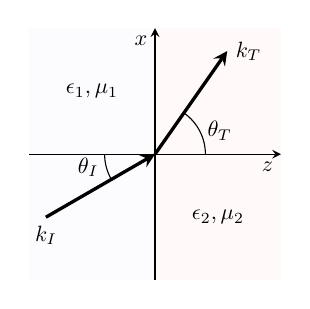
\begin{tikzpicture}[scale = 0.8, every node/.style={scale = 0.8}]
            \fill[Lavender!10] (-2,-2) rectangle (0,2);
            \fill[Pink!10] (0,-2) rectangle (2,2);
            \draw[-stealth] (-2,0) -- (2,0) node[anchor = north east] {\(z\)};
            \draw[-stealth] (0,-2) -- (0,2) node[anchor = north east] {\(x\)};
            \draw[very thick, -stealth] (0,0) -- +(55:2) node[right] {\(\vetor{k}_T\)};
            \draw[very thick, stealth-] (0,0) -- +(210:2) node[below] {\(\vetor{k}_I\)};
            \draw (0.8,0) arc[start angle=0,end angle=55,radius=0.8] node[midway,right] {\(\theta_T\)};
            \draw (-0.8,0) arc[start angle=180,end angle=210,radius=0.8] node[midway, left] {\(\theta_I\)};
            \node at (-1,1) {\(\epsilon_1,\mu_1\)};
            \node at (1,-1) {\(\epsilon_2,\mu_2\)};
        \end{tikzpicture}
    \end{center}
    Em particular, se a luz incide no ângulo crítico
    \begin{equation*}
        \theta_I \to \theta_c = \arcsin\left(\frac{n_2}{n_1}\right),
    \end{equation*}
    então \(\theta_T = \frac{\pi}{2}\), e o raio transmitido simplesmente passa rasante à superfície. Agora, se \(\theta_I\) \emph{exceder} \(\theta_c\), não haverá onda transmitida de forma alguma, somente uma onda refletida (esse é o fenômeno da reflexão interna total, no qual os tubos de luz e as fibras óticas se baseiam). Contudo, mesmo nesse caso, os \emph{campos} não são nulos no meio 2: o que obtemos é a chamada \emph{onda evanescente}, que é rapidamente atenuada e não transporta energia para o meio 2.

    Uma maneira de construir uma expressão para a onda evanescente -- assumindo-se o caso onda há reflexão interna total -- é simplesmente escrever o vetor de onda da onda transmitida como \(\vetor{k}_T = k_T\left(\sin\theta_T \vetor{e}_1 + \cos\theta_T\vetor{e}_3\right)\), onde assumimos que o plano de incidência é o plano \(xz\) e que \(k_T = \frac{\omega n_2}{c}\). Essa estrutura de \(\vetor{k}_T\) pode parecer a mesma que no caso onde não há reflexão interna total. A diferença crucial é que, agora,
    \begin{equation*}
        \sin\theta_T = \frac{n_1}{n_2} \sin\theta_I > \frac{n_1}{n_2} \sin\theta_c = 1.
    \end{equation*}
    Isso pode paracer um absurdo num primeiro momento, e as coisas só se encaixam quando paramos de interpretar \(\theta_T\), nessa particular situação, como um ângulo planar. Mais do que isso, a análise só se torna consistente quando permitimos que \(\theta_T\) seja uma quantidade \emph{complexa}. Muitos textos utilizam notações como \(\tilde{\theta}_T\) para deixar isso claro nesse tipo de contexto. A partir da última relação, temos que
    \begin{equation*}
        \cos\theta_T = i \sqrt{\sin^2\theta_T - 1}
    \end{equation*}
    é uma quantidade puramente imaginária. É importante ressaltar que os campos reais associados à onda evanescente ainda são obtidos tomando as partes reais dos respectivos campos complexos.
    \begin{enumerate}[label=(\alph*)]
        \item Simplesmente utilize a expressão para \(\vetor{k}_T\) para mostrar que
            \begin{equation*}
                \vetor{\tilde{E}}_T = \vetor{\tilde{E}}_T^0 e^{- \kappa z} e^{i(kx - \omega t)},
            \end{equation*}
            onde
            \begin{equation*}
                \kappa = \frac{\omega}{c}\sqrt{(n_1\sin\theta_I)^2 - n_2^2}\quad\text{e}\quad
                k = \frac{\omega n_1}{c}\sin\theta_I.
            \end{equation*}
            Repare que isso representa uma onda que parece se propagar na direção \(x\) (paralela à interface!) e atenuada -- dentro do meio 2 -- na direção \(z\).
        \item Utilizando as relações de Fresnel que você obteve no \cref{ex:exercício04}, no caso da polarização perpendicular ao plano de incidência, calcule o coeficiente de reflexão para uma situação onde há reflexão interna total num problema de incidência com essa mesma polarização. Interprete fisicamente.
        \item Ainda no mesmo contexto do item (b), mostre que os campos reais associados à onda evanescente são
            \begin{align*}
                \vetor{E}_T(\vetor{\x},t) &= E_0^T e^{- \kappa z} \cos(kx - \omega t) \vetor{e}_2
                \quad\text{e}\quad\\
                \vetor{B}_T(\vetor{\x},t) &=\frac{E_0^T}{\omega}e^{- \kappa z} \left[\kappa \sin(kx - \omega t)\vetor{e}_1 + k\cos(kx - \omega t) \vetor{e}_3\right],
            \end{align*}
            e verifique que eles satisfazem todas as equações de Maxwell.
        \item Considerando os campos acima, construa o vetor de Poynting e mostre que, na média sobre o período de uma oscilação, não há transmissão de energia na direção \(z\).
    \end{enumerate}
\end{exercício}
\begin{proof}[Resolução]
    Com as definições feitas, temos
    \begin{align*}
        \vetor{k}_T &= k_T \left(\sin\theta_T \vetor{e}_1 + i \sqrt{\sin^2\theta_T - 1}\vetor{e}_3\right)\\
                    &= \frac{k_T}{n_2} \left(n_1\sin\theta_I \vetor{e}_1+ i\sqrt{n_1^2 \sin^2 \theta_I - n_2^2}\vetor{e}_3\right)\\
                    &= \frac{\omega}{c}\left(n_1 \sin\theta_I \vetor{e}_1 + i \sqrt{n_1^2 \sin^2 \theta_I - n_2^2}\vetor{e}_3\right).
    \end{align*}
    Assim, escolhendo a fase de \(\tilde{E}_T^0\) de forma que \(\tilde{E}_T^0 = E_T^0\) para simplificar, o campo elétrico é dado por
    \begin{equation*}
        \vetor{\tilde{E}}_T = \vetor{\tilde{E}}_T^0 e^{i(\vetor{k}_T \cdot \vetor{\x} - \omega t)} = \vetor{\tilde{E}}_T^0 e^{-\kappa z} e^{i(k x - \omega t)} = E_T^0 e^{-\kappa z}e^{i(kx - \omega t)}\vetor{e}_2,
    \end{equation*}
    onde \(\vetor{k}_T = k \vetor{e}_1 + i\kappa\vetor{e}_3\).

    Tomando o caso da incidência com polarização ortogonal ao plano de incidência, temos do \cref{ex:exercício04} que
    \begin{equation*}
        R = \abs*{\frac{1 - \alpha \beta}{1 + \alpha \beta}}^2 = \frac{(1 - \conj{\alpha} \beta)(1 - \alpha \beta)}{(1 + \conj{\alpha}\beta)( 1 + \alpha \beta)} = \frac{(1 + \alpha \beta) ( 1 - \alpha \beta)}{(1 - \alpha \beta)( 1 + \alpha \beta)} = 1,
    \end{equation*}
    já que \(\alpha\) é puramente imaginário. Desse modo, como \(R + T = 1\), sabemos que \(T = 0\), portanto espera-se que, em média, não haja transferência de energia para o meio 2, o que mostraremos a seguir.

    Antes de prosseguir, mostremos que os campos reais satisfazem as equações de Maxwell. O campo magnético é dado por
    \begin{equation*}
        \vetor{\tilde{B}} = \frac1\omega\vetor{k}_T\times \vetor{\tilde{E}}_T = \frac{1}{c} E_T^0 e^{- \kappa z}e^{i(kx - \omega t)}\left(n_1\sin\theta_I \vetor{e}_3 - i\sqrt{n_1^2 \sin^2\theta_i - n_2^2}\vetor{e}_1\right),
    \end{equation*}
    logo os campos reais são dados por
    \begin{equation*}
        \vetor{E}_T = E_T^0 e^{- \kappa z} \cos(kx - \omega t)\vetor{e}_2,\quad\text{e}\quad
        \vetor{B}_T = \frac{E_T^0}{\omega} e^{- \kappa z}\left[\kappa \sin(k x - \omega t) \vetor{e}_1 + k \cos(kx - \omega t) \vetor{e}_3\right].
    \end{equation*}
    É fácil ver que os divergentes dos campos se anulam, pois
    \begin{equation*}
        \nabla \cdot \vetor{E}_T = \diffp{\inner{\vetor{e}_2}{\vetor{E}_T}}{y} \vetor{e}_2 \cdot \vetor{e}_2 = 0,\quad\text{e}\quad
        \nabla \cdot \vetor{B}_T = \diffp{\inner{\vetor{e}_2}{\vetor{B}_T}}{y} \vetor{e}_2 \cdot \vetor{e}_2 = 0.
    \end{equation*}
    Verifiquemos a lei de Faraday,
    \begin{align*}
        \nabla \times \vetor{E}_T &= -\diffp{\inner{\vetor{e}_2}{\vetor{E}_T}}{z}\vetor{e}_1 + \diffp{\inner{\vetor{e}_2}{\vetor{E}_T}}{x}\vetor{e}_3 \\
                                &= E_T^0e^{- \kappa z}\left(\kappa \cos(kx - \omega t)\vetor{e}_1 + k \sin(k x - \omega t) \vetor{e}_3\right)\\
                                &= - \diffp{\vetor{B}_T}{t}.
    \end{align*}
    Por fim, temos
    \begin{align*}
        \nabla \times \vetor{B}_T &= \left(\diffp{\inner{\vetor{e}_1}{\vetor{B}_T}}{z} - \diffp{\inner{\vetor{e}_3}{\vetor{B}_T}}{x}\right) \vetor{e}_2\\
                                &= \frac{E_T^0}{\omega} e^{- \kappa z}\left[-\kappa^2 \sin(k x - \omega t) + k^2 \sin(kx - \omega t)\right]\vetor{e}_2\\
                                &= -\frac{E_T^0 n_2^2 \omega}{c^2} e^{- \kappa z} \sin(k x - \omega t) \vetor{e}_2\\
                                &= \frac{n_2^2}{c^2} \diffp{\vetor{E}_T}{t}\\
                                &= \mu_2 \epsilon_2 \diffp{\vetor{E}_T}{t},
    \end{align*}
    portanto os campos satisfazem as equações de Maxwell.

    O vetor de Poynting é dado por
    \begin{align*}
        \vetor{S}_T = \frac1{\mu_2}\vetor{E}_T\times \vetor{B}_T
        &= \frac{1}{\mu_2 \omega} (E_T^0)^2 e^{- 2 \kappa z} \cos(kx - \omega t) \left[- \kappa \sin(kx - \omega t) \vetor{e}_3 + k \cos(kx - \omega t)\vetor{e}_1\right]\\
        &= \frac{1}{\mu_2 \omega} (E_T^0)^2 e^{-2 \kappa z} \left[k \cos^2(kx - \omega t) \vetor{e}_1 - \kappa \cos(kx - \omega t)\sin(kx - \omega t)\vetor{e}_3\right],
    \end{align*}
    portanto
    \begin{equation*}
        \mean{\vetor{e}_3\cdot\vetor{S}_T} = 0
    \end{equation*}
    segue da ortogonalidade de senos e cossenos.
\end{proof}
